%% Sample file for a Modelica Conference user-presentation one-pager
%% Copyright Modelica Association
%
% This work may be distributed and/or modified under the
% conditions of the LaTeX Project Public License, either version 1.3
% of this license or (at your option) any later version.
% The latest version of this license is in
%   http://www.latex-project.org/lppl.txt
% and version 1.3 or later is part of all distributions of LaTeX
% version 2005/12/01 or later.
%
% This work is 'maintained' on GitHub:
%   https://github.com/modelica-association/conference-templates
%
% Use this template for industrial / user presentations that are
% listed in the conference programme but are not scientific papers.
% The result must fit on a single A4 page.

%%% Class option 'userpresentation': single column, same margins/fonts/title
%%% layout as scientific papers. Bibliography defaults to biber/biblatex.
\documentclass[userpresentation]{modelica}
\addbibresource{example-user-presentation.bib}

\hypersetup{%
  pdftitle  = {User Presentation One-Pager Template for a Modelica Conference},
  pdfauthor = {Author Name1, Author Name2},
  pdfsubject = {Modelica Conference -- User Presentation},
  pdfkeywords = {Modelica, conference, user presentation, one-pager, LaTeX, template},
  colorlinks,
  linkcolor=black,
  urlcolor=black,
  citecolor=black,
  pdfpagelayout = SinglePage,
  pdfcreator = pdflatex,
  pdfproducer = pdflatex
}

\usepackage[utf8]{inputenc}

\begin{document}
\thispagestyle{empty}

%%----------------------------------------------------------------------
%% Title and authors -- same style as scientific papers
%% Capitalize words in the title. Keep the list of authors short.
%%----------------------------------------------------------------------
\title{User Presentation One-Pager: Title of Your Industrial Talk}
\author[1]{Author Name}
\author[1]{Author Name}
\author[2]{Author Name}
\affil[1]{Company or Department, Organization, Country, {\small\texttt{\{name1,name2\}@company.org}}}
\affil[2]{Company, Country, {\small\texttt{name3@company.org}}}

\maketitle\thispagestyle{empty} %% required on the first (and only) page

%%----------------------------------------------------------------------
%% Recommended figure (optional but strongly encouraged)
%% Place a single, wide illustration after the title block so programme
%% readers can grasp the topic at a glance: product photo, plant schematic,
%% simulation screenshot, architecture diagram, key result plot, \ldots
%% Prefer vector graphics (PDF/SVG/EPS) over raster images when possible.
%% Do not use a floating placement that can push content to a second page;
%% keep the figure in the reading flow (as below) and size it carefully.
%%----------------------------------------------------------------------
\begin{center}
  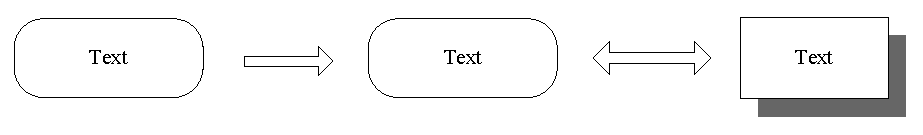
\includegraphics[width=0.92\textwidth]{resources/figure2}
  \captionof{figure}{Recommended overview figure (replace with your own).
    Typical choices: application photo, system schematic, tool screenshot,
    or a plot of the main result discussed in the talk.}
  \label{fig:overview}
\end{center}

%%----------------------------------------------------------------------
%% Presentation abstract -- no "Abstract" heading
%% Write a concise description of the talk for the conference programme.
%% Goal: help attendees decide whether to attend. Cover motivation,
%% industrial context, what will be shown, and take-away messages.
%% Do not structure this one-pager like a full scientific paper
%% (no Introduction/Methods/Results sections). Plain paragraphs only.
%% Strict length limit: everything on this page, including any references.
%%----------------------------------------------------------------------
\noindent
This document is the official one-page template for \emph{user presentations}
at a Modelica Conference. A user presentation is
\emph{not} a scientific publication. It is typically given by an industrial
user, tool vendor, or practitioner and is announced in the conference
programme. This single page is what participants read when choosing sessions:
keep it informative, concrete, and easy to skim.

\vspace{0.6ex}
\noindent
\textbf{Layout rules (already built into the class).}
Title, author block,
fonts (Times-like body text at 10.5\,pt), and page margins match the
scientific paper template. Unlike papers, the layout is
\emph{single-column over the full text width}. There is no separate
abstract heading: the text after the optional figure \emph{is} the abstract
of the presentation. Optional references may appear at the bottom; because
this is not a research paper, prefer links to software, standards, product
pages, or a few closely related publications rather than a full literature
survey~\cite{modelicaOrg,fmiStandard}.

\vspace{0.6ex}
\noindent
\textbf{What to write.} State the industrial problem or use case, the role of
Modelica/FMI or related technology, what the audience will see in the talk
(demo, case study, lessons learned, deployment experience), and the main
conclusions or open challenges. Replace this instructional wording with your
own content. Keywords are optional; if used, keep them on one short line as
in the scientific template.

\vspace{0.6ex}
\noindent
\emph{Keywords: user presentation, industrial application, Modelica, FMI}

%%----------------------------------------------------------------------
%% Optional references -- software links and closely related work
%% Omit \printbibliography entirely if you have nothing useful to list.
%% Keep the list short so the page does not overflow.
%%----------------------------------------------------------------------
\printbibliography[title=References]

\end{document}
